\documentclass[
	a4paper, % Paper size, use either a4paper or letterpaper
	12pt, % Default font size, the template is designed to look good at 12pt so it's best not to change this
	%unnumberedsections, % Uncomment for no section numbering
]{article}
\usepackage[a4paper,top=0.4cm, bottom=0.8cm, left=1.6cm, right=1.6cm]{geometry}

\usepackage{cmap} % make PDF files searchable and copy-able
\usepackage[utf8]{inputenc}
\usepackage[english,russian]{babel}

\usepackage{amssymb,amsmath}
\renewcommand {\phi}{\varphi}
\usepackage{mathtext}

\usepackage{libertine}
\usepackage[libertine]{newtxmath}

\usepackage{graphicx} % Required for inserting images
\graphicspath{{./img/}} % Destination of images
\usepackage{subcaption}

\usepackage{hyperref}

\usepackage{xcolor}



% opening
\title{
	\textcolor{cyan}{Отчет о выполнении лабораторной работы 1.1.7}
	\\
	Экспериментальное исследование равноускоренного движения
}
\author{Шубин Владислав, Байбулатов Амир}
%\date{Сентябрь 2023}

\begin{document}    
	
	\maketitle
	
	\section{Аннотация}
	В данной работе исследуется равноускоренное движение на примере магнита, скользящего по внутренней поверхности наклонной пластиковой трубы (\ref{fig:subim2}). Регистрация положения магнита в зависимости от времени осуществляется электромагнитными датчиками(система катушек). Все катушки соединены последовательно. Прохождение магнита через каждую катушку приводит, ввиду явления электромагнитной индукции, к генерации импульса напряжения во всей цепи, который замеряется блоком регистрации сигнала. Масса груза измеряется весами, координаты катушек измеряются линейкой. Детально исследуется систематические и случайные погрешности проводимых измерений.
	
	
	\section{Теоретические сведения}
	
	\subsection{Метод самоиндукции}
	
	\begin{figure}[h]
		\begin{subfigure}{0.5\textwidth}
			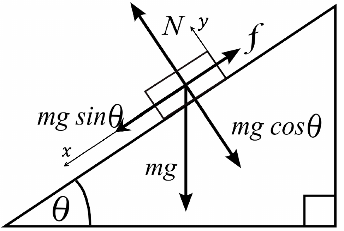
\includegraphics[width=0.9\linewidth]{scheme.png} 
			\caption{К выводу закона движения\\ по наклонной плоскости}
			\label{fig:subim1}
		\end{subfigure}
		\begin{subfigure}{0.5\textwidth}
			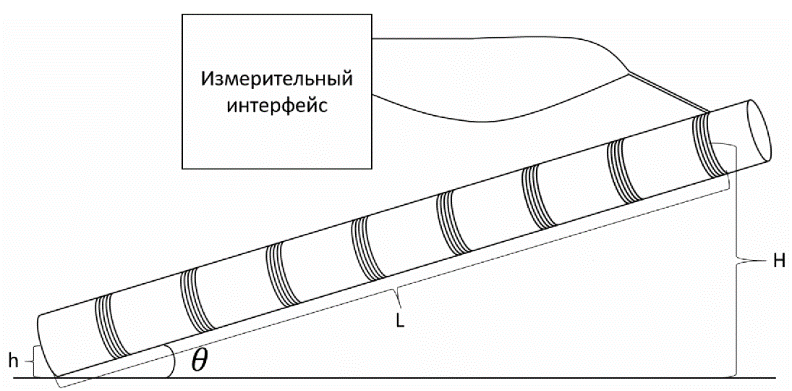
\includegraphics[width=0.9\linewidth]{tube.png}
			\caption{Экспериментальная установка}
			\label{fig:subim2}
		\end{subfigure}
	\end{figure}
	
	Запишем второй закон Ньютона в проекциях на наклонную плоскость $(ось Ox)$ и перпендикуляр к ней $(ось Oy)$, см. \ref{fig:subim1}:
	\begin{equation}
		Ox: ma = mg\sin{\theta} - f,
		\label{first}
	\end{equation}
	\begin{equation}
		Oy: \:\:\:\:\:\:\:\:\:N = mg\cos{\theta}.
		\label{second}
	\end{equation}
	
	Здесь $\theta$ — угол наклона плоскости к горизонту, $f$ — сила трения, $a$ — ускорение тела, $N$ — сила реакции опоры, $g$ — ускорение свободного падения.
	Сила трения $f$ состоит из сопротивления воздуха и силы трения о плоскость. Можно предположить, что основной вклад в
	силу трения вносит сухое трение, пропорциональное силе реакции опоры.
	Тогда $f$ = $\mu$ , где $\mu$ — коэффициент трения скольжения, зависящий только от свойств материалов.
		
	Решая систему \ref{first} и \ref{second}, получим выражение для ускорения:
	\begin{equation}
		a = g(\sin{\theta} - \mu\cos{\theta})
	\end{equation}
	
	Закон прямолинейного равноускоренного движения вдоль оси Ox, как известно, имеет вид:
	\begin{equation}
		x = v_{0}t + \frac{at^{2}}{2},
	\end{equation}
	где $x$ — координата тела, $v_0$ — начальная скорость (скорость в точке $x=0$).
	
	При приближении магнита к катушке поле вблизи катушки (а значит и его поток)
	сначала нарастает (по модулю), достигает максимума в средней точке, и затем, по мере удаления магнита, убывает до нуля. Исследуемый сигнал имеет два экстремума: последовательные максимум и минимум с прохождением через 0 (см \ref{fig:subim3}) Зависимость напряжения в цепи катушек от времени представляет собой набор пиков (см. \ref{fig:subim4})
	
	\begin{figure}[h]
		\begin{subfigure}{0.5\textwidth}
			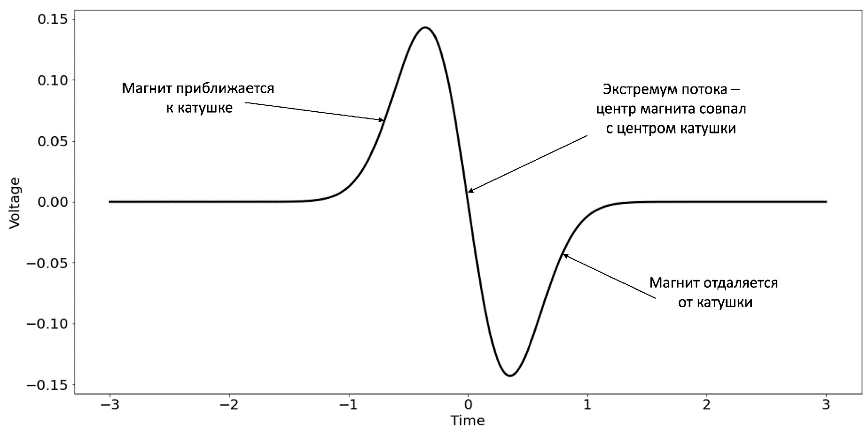
\includegraphics[width=0.9\linewidth]{once.png} 
			\caption{Зависимость напряжения от времени при пролёте магнита через одну катушку}
			\label{fig:subim3}
		\end{subfigure}
		\begin{subfigure}{0.5\textwidth}
			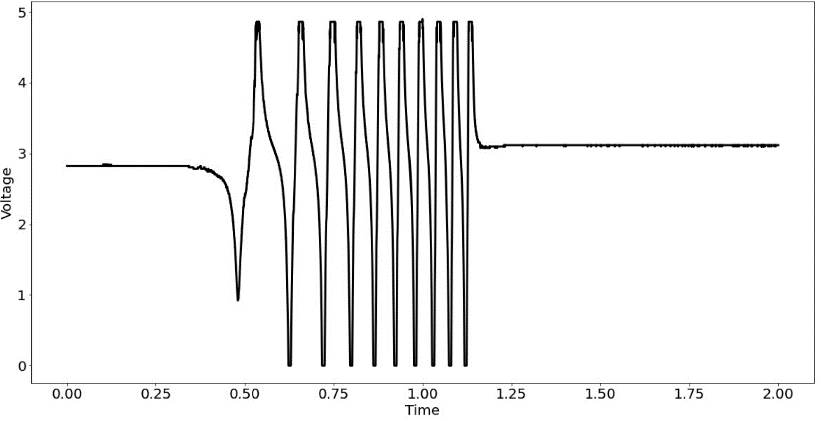
\includegraphics[width=0.9\linewidth]{multi.png}
			\caption{Пример сигнала при пролёте магнитом 10 катушек}
			\label{fig:subim4}
		\end{subfigure}
	\end{figure}
	
	Далее определяются параметры $v_0$ и $a$, при которых зависимость (\ref{fig:subim4}) наилучшим образом накладывается на экспериментальные точки.
	
	Используется численный \textit{метод наименьших квадратов}:
	\begin{equation}
		S = \sum_{n}\big(x_n - v_{0}t_{n} - \frac{at_{n}^{2}}{2}\big)^2 \rightarrow \min
	\end{equation}
	
	По результатам серии экспериментов при разных углах из пар значений {$a$, $\theta$} тем же методом наименьших квадратов для теоретической зависимости (\ref{fig:subim3}) определяются параметры ускорение свободного падения $g$ и коэффициент трения $\mu$.
	Для линеаризации зависимости (\ref{fig:subim3}) можно использовать, например, замену
	\begin{equation}
		a' = \frac{a}{\cos{\theta}}
	\end{equation}
	
	\begin{equation}
		\tau = \tg{\theta}
	\end{equation}
	
	Тогда
	\begin{equation}
		a' = g(\tau - \mu)
	\end{equation}
	
	\section{Оборудование и инструментальные погрешности}
	\textbf{Оборудование:} труба с намотанными катушками, фиксируемая на штативе; неодимовые магниты; линейка; блок регистрации сигнала (усилитель + микроконтроллер с АЦП), соединённый с компьютером.
	\begin{itemize}
		\item \textbf{Линейка}: $\Delta \text{лин} = \pm0.1$ см (по цене деления)
		\item \textbf{Весы}: $\Delta m = \pm{5}$ мг (маркировка производителя)
	\end{itemize}
	
	\newpage
	
	\section{Результаты измерений и обработка данных}
	
	\subsection{Характеристики системы:}
	
	$m = 3.589\pm 0,005$ г,\\
	
	\begin{table}[h]
		\centering
		\begin{tabular}{|c|c|c|c|c|c|c|c|c|c|c|}
			\hline
			N катушки & 1 & 2 & 3 & 4 & 5 & 6 & 7 & 8 & 9 & 10  \\
			\hline
			x, см & 0.0 & 10.2 & 20.1 & 30.1 & 40.1 & 50.1 & 60.1 & 70.1 & 80.2 & 90.0 \\
			\hline
		\end{tabular}
		\caption{Результаты измерений координат катушек.}
		\label{table:1}
	\end{table}
	
	\subsection{Измерения:}

	
	%\newpage
	
	\begin{table}[h]
		\centering
		\begin{tabular}[H]{|c|c|c|c|c|c|}
			\hline
			\textnumero & $\theta$, град & $a_{\min},\frac{\text{м}^2}{\text{с}^2}$ & $a_{\max},\frac{\text{м}^2}{\text{с}^2}$ & $\sigma_{\min},\frac{\text{м}^2}{\text{с}^2}$ & $\sigma_{\max},\frac{\text{м}^2}{\text{с}^2}$  \\
			\hline
			1 &  &  &  &  &   \\
			\hline
			2 &  &  &  &  &    \\
			\hline
			3 &  &  &  &  &    \\
			\hline
			4 &  &  &  &  &   \\
			\hline
			5 &  &  &  &  &   \\
			\hline
			6 &  &  &  &  &    \\
			\hline
			7 &  &  &  &  &    \\
			\hline
			8 &  &  &  &  &   \\
			\hline
			9 &  &  &  &  &   \\
			\hline
			10 &  &  &  &  &    \\
			\hline
			11 &  &  &  &  &    \\
			\hline
			12 &  &  &  &  &   \\
			\hline
			13 &  &  &  &  &   \\
			\hline
			14 &  &  &  &  &    \\
			\hline
			15 &  &  &  &  &    \\
			\hline
			16 &  &  &  &  &   \\
			\hline
			17 &  &  &  &  &    \\
			\hline
			18 &  &  &  &  &   \\
			\hline
		\end{tabular}
		\caption{Результаты измерений ускорений при различных углах.}
		\label{table:2}
	\end{table}
	\begin{table}[h]
		\centering
		\begin{tabular}[H]{|c|c|c|c|c|c|c|c|c|c|c|}
			\hline
			$\Delta x_{\text{ср}}$, мм & 12.5 & 11.5 & 11.8 & 11.4 & 11.9 & 12.2 & 11.7 & 11.1 & 11.0 & 12.0  \\
			\hline
			$u$, м/c & 148.0 & 136.4 & 143.3 & 138.2 & 143.4  & 145.5 & 140.7 & 133.7 & 132.0 & 146.3  \\
			\hline
		\end{tabular}
		\caption{Результаты вычислений скорости пули.}
		\label{table:3}
	\end{table}
	
	Рассчитаем систематическую и случайную погрешности:
	\begin{equation}
		\sigma_u^{\text{сист}} =u \sqrt{\varepsilon_M^2 + \varepsilon_m^2 + \varepsilon_{\Delta x}^2 + \left(\frac{\varepsilon_L}{2} \right)^2}  \;\;\;\;\; \sigma_u^{\text{случ}} = \sqrt{ \frac{1}{n(n-1)} \sum_{i=1}^{n}(u_i - u_{\text{ср}})^2} \;\;\;\;\; \sigma_u =\sqrt{\sigma_{\text{сист}}^2 + \sigma_\text{случ}^2} 
	\end{equation}
	\begin{equation}
		\sigma_u^\text{сист}\approx 3,8 \text{ }\dfrac{\text{м}}{\text{с}} \;\;\;\;\;\;\;\;\;\;\;\;\;\;\;\;\;\;\;\;\;\;\;\;\;\;\;\;\;\;\; \sigma_u^\text{случ}\approx 1,7 \text{ }\dfrac{\text{м}}{\text{с}} \;\;\;\;\;\;\;\;\;\;\;\;\;\;\;\;\;\;\;\;\;\;\;\;\;\;\;\;\;\;\;
		\sigma_u \approx 4,2 \text{ }\dfrac{\text{м}}{\text{с}}
	\end{equation}
	
	\section{Заключение}
	В ходе эксперимента получены величины ускорения свободного падения g и коэффициент трения скольжения $\mu$ трубы. Получилось, что ускорение свободного падения с точность до погрешности равна g = 9.81, что подтверждает применимость законов Ньютона на практике.
	Значение, посчитанное по точкам максимума оказалось больше значения g = 9.81.
	Это можно объяснить лишь неаккуратным запуском магнита с приданием ему началь-
	ной скорости, т.к. иные источники погрешностей будут давать отклонение в меньшую
	сторону.
	
	
\end{document}
